\documentclass[11pt]{article}
\usepackage[small,compact]{titlesec}
\usepackage[margin=0.25in]{geometry}
\usepackage{subcaption}
\usepackage{common}
\title{\begin{center}
{\Large Practical 4: Reinforcement Learning}
\end{center}}
\author{ Baojia Tong (baojia.tong@cern.ch)\\Yuliya Dovzhenko (dovzhenko@g.harvard.edu)\\Alan Legoallec (alanlegoallec@g.harvard.edu )\\\\Public Repository: https://github.com/tongbaojia/pubcs181}
\begin{document}
\maketitle{}
The goal of this assignment is to program an agent that learns to play the game Swingy Monkey. Agent's actions are either jump or no jump. 
\section{Method}
We have tried the following methods: Deterministic policy, $\epsilon$-greedy Q learning, Q learning with Neural Net basis, Q learning with analytical function basis.We were able to achieve an average score of above 10 after 100 epochs, averaged over ten iterations. However, performance varied significantly from iteration to iteration and epoch to epoch.
\subsection{Fixed Policy}
\paragraph{}
There exists simple analytical solutions to this problem, if the speed change every time is not Poisson. Given this randomness nature, the solution can no longer be deterministic. However, if the gravity is large, thus the speed change could be compensated over a certain time, a simple solution could still be achieved, as shown in Figure ~\ref{FixedPolicy}. This is coded as the "$tran\_model$" function.
\begin{figure}[] 
\centering
        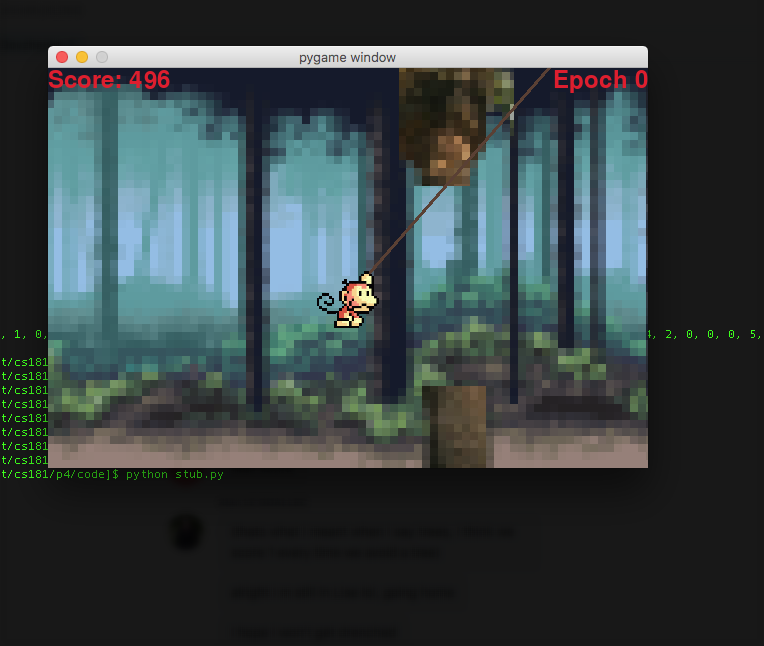
\includegraphics[width=0.33\textwidth]{Plot/highscore.png}
        \caption{In high g environment, a simple method gives an endless game; first trial can get to 496+.}
            \label{FixedPolicy}
\end{figure}
\subsection{Q-learning}
\paragraph{}
We tried off-policy method to fully explore the world.
\paragraph{Inputs} We used tree distance, monkey velocity, monkey top position and monkey-tree bottom difference to describe the state, and jump or not as action. Extra dimensions could be useful but also may be costly in training, since then the parameter space gets large. 
\paragraph{Initialization}Figure ~\ref{QInitial} demonstrates that given the same variables, different initiation and binning can have very different learning behavior. Given the same length of game trials, a better initialization would give more reward-action iterations and hence increase the learning effect.
\begin{figure}[] 
\centering
        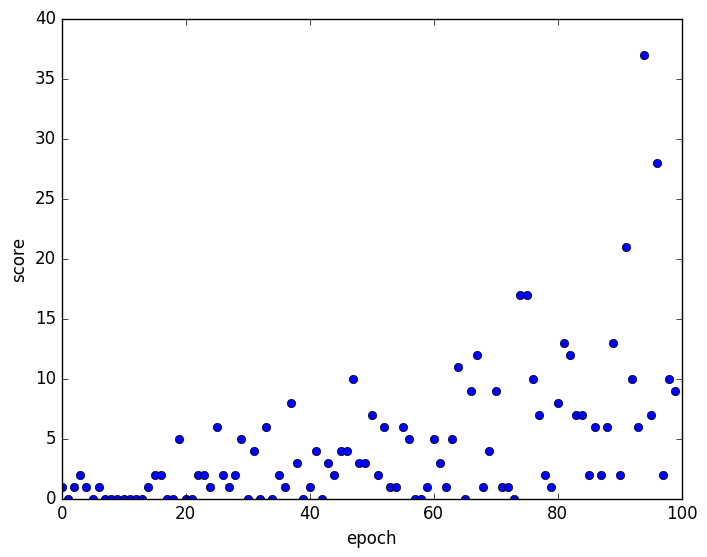
\includegraphics[width=0.33\textwidth]{Plot/learn_vel5_mtop25.png}
        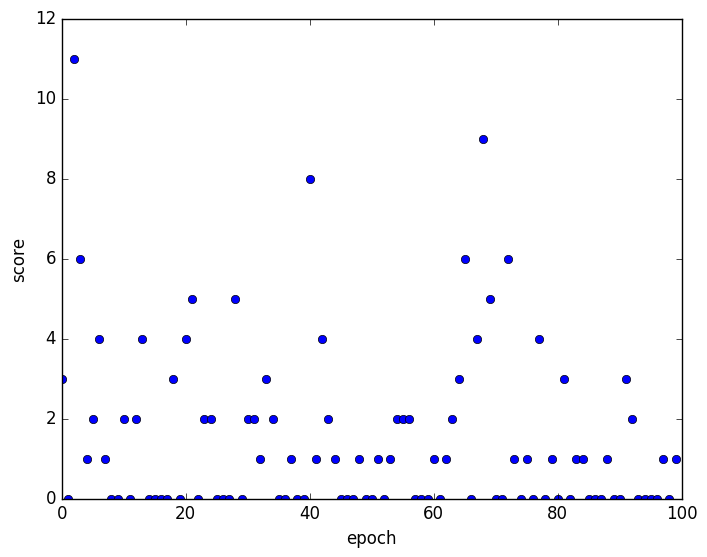
\includegraphics[width=0.33\textwidth]{Plot/learn_vel10_mtop50.png}
        \caption{In high gravity case, learning score as a function of games. Left: initialization with velocity bin size of 5 and monkey top size of 25; right: initialization with velocity bin size of 10 and monkey top size of 50.}
            \label{QInitial}
\end{figure}
\paragraph{Learning Parameters} affect the learning rate. For example, the exploration factor is described by the parameter $\epsilon$. For a larger $\epsilon$, in the early learning stage it helps to explore more states, and thus helpful for the performance. This is shown in Figure ~\ref{Qepsilon}.
\begin{figure}[] 
\centering
        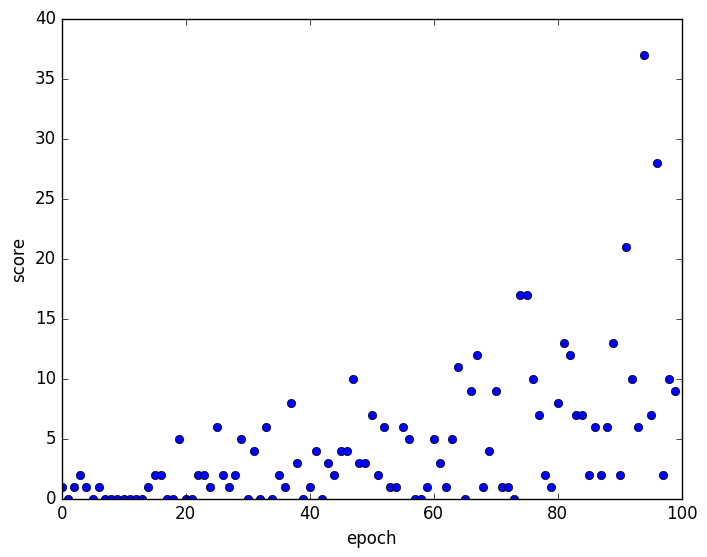
\includegraphics[width=0.33\textwidth]{Plot/learn_vel5_mtop25.png}
        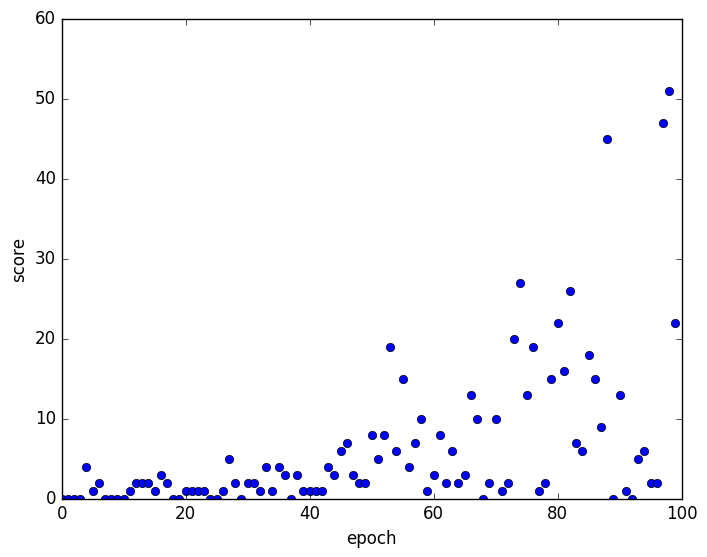
\includegraphics[width=0.33\textwidth]{Plot/learn_epsilon01.png}
        \caption{In high gravity case, learning score as a function of games. Left: initialization with $\epsilon$ of 0.001 ; right: initialization with $\epsilon$ of 0.1. Notice the y-axis increase in the larger epsilon case.}
            \label{Qepsilon}
\end{figure}
%%Tony: This paragraph could be commented out. It is very hard for me to understand this as well.
\paragraph{Modeling} for different gravity world maybe not be the same. Therefore we tried two different Q matrices, one for low gravity and one for high gravity--they have the same input parameters but different initializations. Once a new state is available, which gravity world we are in could be determined by the monkey's velocity difference. Then the corresponding Q matrix is used to learn and predict the world. In general, the low gravity case is harder to model because the randomness in the impulse will have a larger effect in the next states. This is shown in Figure ~\ref{QModel}.
\begin{figure}[] 
\centering
        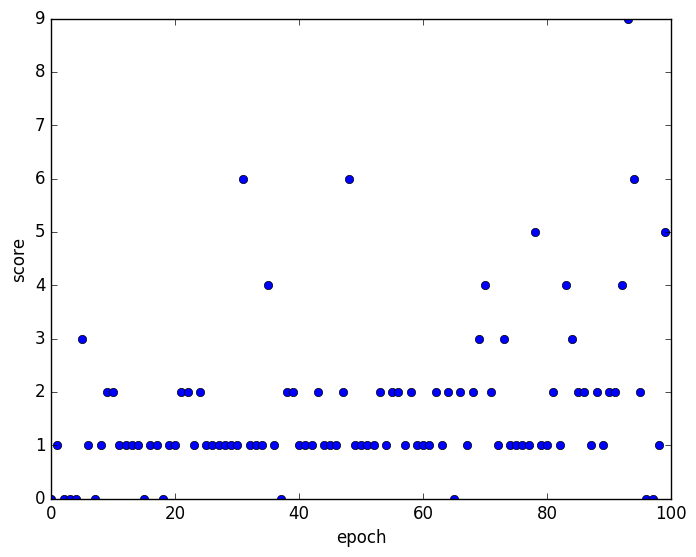
\includegraphics[width=0.3\textwidth]{Plot/learn_lowonly2.png}
        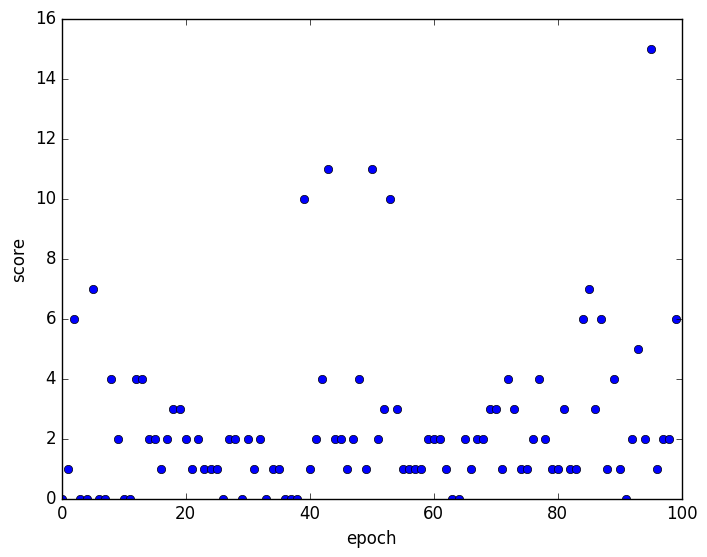
\includegraphics[width=0.3\textwidth]{Plot/learn_highonly2.png}
        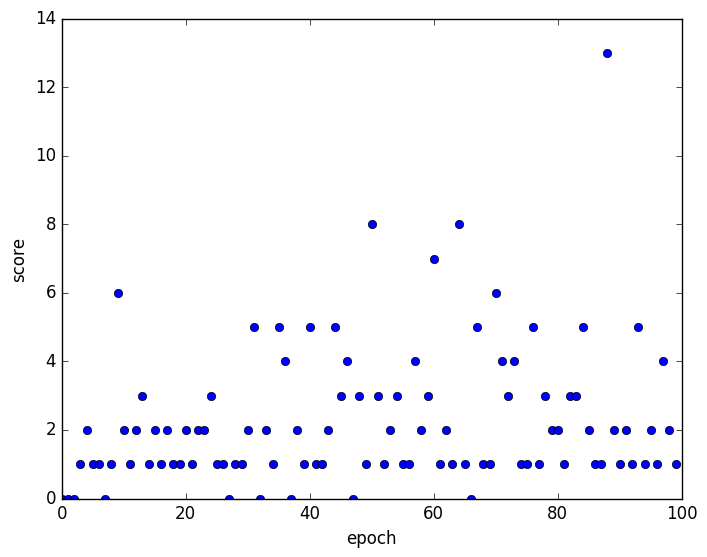
\includegraphics[width=0.3\textwidth]{Plot/learn_mix.png}
        \caption{Left: with the low G model only; middle: with the high G model only; right: with the mixed model.}
            \label{QModel}
\end{figure}
\subsection{Neural Net Basis}
Our main challenge is the size of the state space. We can round distances to a coarse grid, potentially throwing away useful information. The state space is still large. Furthermore, we don't take advantage of the physical simplicity of the problem. We would like the monkey to see that a new state may be very similar to a known state.
\\One approach is to treat $Q(s,a)$ as an adaptive function of the inputs, i.e. neural net. Ideally, we would perform steepest gradient descent to optimize the parameters of the net. We would need to compute $\frac{\partial Q}{\partial w}$ for each $w$ parameter of the net. Given the time constraints, we chose to use a scikit multilayer perceptron library. Instead of performing steepest descent, we take a weighted average of current prediction $Q(s,a)$ with newly obtained information:
\begin{equation}Q(s,a)\rightarrow(1-\eta)Q(s,a)+\eta(r(s,a)+\gamma\max_{a'}Q(s',a'))\label{eq}\end{equation}
We trained the neural net after each game on a limited history of past $(s,a)$ pairs and corresponding $Q(s,a)$ values from eq. \ref{eq}. Once the net is trained, we use it to estimate $Q(s,a)$ in the next game. We limited the maximum history length to speed up the training, as well as to discard old data in favor of new data. Average score as function of history size is plotted in Fig. \ref{nn} (left). Like the previous method, this one performed much better in high gravity than low gravity, see for example a histogram of scores from one run in Fig. \ref{nn} (right).
\begin{figure}[] 
\centering
        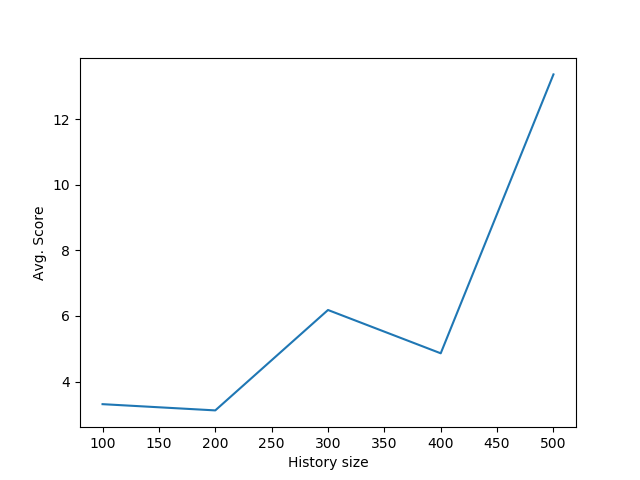
\includegraphics[width=0.35\textwidth]{NN_plots/History_size.png}
        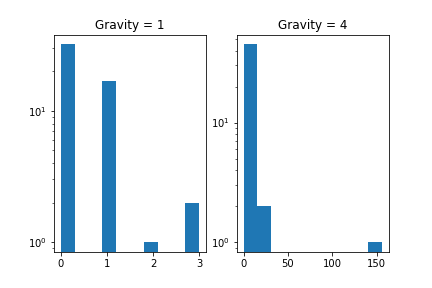
\includegraphics[width=0.4\textwidth]{NN_plots/NN_layers_5_5_eps_0_g_0_9_iter_100_histograms.png}
        \caption{Left: Average score after 100 epochs repeated 10 times using a neural net basis as function of history size. History size determines maximum number of past state-action pairs used to train the neural net. Right: Histogram of scores using a neural net basis grouped by gravity.}
            \label{nn}
\end{figure}
\subsection{Analytical Basis Functions} 
The objective here is to condense a large parameter space to fewer relevant quantities. We tried to express $Q(s,a)$ in a time basis (converting distances into time to collision). For example, here is how we solve for time until monkey hits the ground:
\begin{gather}
%-d_{ground} = -\frac{1}{2}gt^2+vt\\
t = \frac{v+\sqrt{v^2-2gd_{ground}}}{g},
\end{gather}
Solving for time until hitting the roof and time to next tree in a similar fashion, we put forward the following functional forms for $Q(s,0)$ and a similar one for $Q(s,1)$:
\begin{gather}
Q(v, g, d_{ground},d_{front}, a= 0) = A\frac{v}{g}+B\frac{\sqrt{v_0^2-2gd_{ground}}}{g}+Cd_{front},\\
%Q(v, g, d_{top},d_{front}, a=1) = E\frac{v}{g}+E\frac{\sqrt{v_0^2+2gd_{top}}}{g}+Fd_{front}
\end{gather}
where $A,B,C$ are parameters to be tuned via steepest descent. %Here is an example of an update to $A$:
%\begin{equation}
%A\leftarrow A-\eta(Q(s,a)-r(s,a)-\gamma\max_{a'}Q(s',a'))\frac{\partial Q}{\partial A}
%\end{equation}
\\In practice this method led to rapidly diverging values of the coefficients, even with small $\eta$. A possible reason is that this model for $Q(s,a)$ is over-simplified.
\subsection{Undetermined gravity
}
Each gravity can be trained separately, using the value of the gravity as a state. As mentioned above, gravity can easily be determined if the monkey is not jumping. There are several ways to deal with the incertitude at the beginning of each epoch.
1-Enforce that the first move of the monkey should be not to jump, to infer the gravity, and then only train/use the model. 
2-Encode the unknown gravity as a 5th value of the state (e.g zero), which can be used/trained until the gravity is determined for this epoch.
3-Use the most likely gravity, correcting for the effect of the impulse, whose distribution parameter is known (Poisson(15)), until the actual gravity can be determined.
4-Start with an arbitrary value of the gravity, close to the average/median. (2 or 3)
\section{Discussion} 
For each method, we found it difficult to achieve consistent performance across different epochs. One reason is that low gravity is harder to beat. In Fig. \ref{nn}, we show histograms for two different gravity values an the difference is significant.
\\With a neural net basis, we were able to achieve an average score of over 10 after 100 epochs. However, the performance varied greatly from iteration to iteration and from epoch to epoch. In order to obtain average scores, we ran 100 epochs 10 times. The neural net method was also slow due to the need to train the net at every iteration. History size was a challenge: we want a moving window, in order to forget earlier values, but we also need a lot of data to train the net. 

\end{document}

